% !TEX root = ../main.tex
\section{Ejercicio propuesto 1: implementación y validación del Link-Cut Tree}

\subsection{Estructura de punteros y métodos internos clave}
Cada vértice se modela con \texttt{LinkCutNode}. Los auxiliares son Splay Trees que almacenan los caminos preferidos. El puntero \texttt{parent} cumple dos roles: une nodos dentro del auxiliar y, en la raíz auxiliar, actúa como \textbf{puntero virtual o \textit{path-parent}} hacia el nodo superior del camino lógico. La raíz auxiliar se reconoce porque su padre no la referencia como hijo:

\begin{lstlisting}[language=Python, caption={Métodos internos críticos: raíz auxiliar, propagación lazy y agregados}, label={lst:lct_internos}]
def _is_aux_root(self, x: LinkCutNode) -> bool:
    p = x.parent; return p is None or (p.left is not x and p.right is not x)

def _push(self, x: Optional[LinkCutNode]):
    if x and x.reversed:
        x.left, x.right = x.right, x.left
        if x.left:  x.left.reversed = not x.left.reversed
        if x.right: x.right.reversed = not x.right.reversed
        x.reversed = False; self.stats.lazy_reversals += 1

def _update(self, x: LinkCutNode):
    x.size = 1 + (x.left.size if x.left else 0) + (x.right.size if x.right else 0)
    x.path_sum = x.value + (x.left.path_sum if x.left else 0) + (x.right.path_sum if x.right else 0)
    self.stats.updates += 1
\end{lstlisting}

\subsection{Operaciones del bosque dinámico}
\begin{itemize}\setlength\itemsep{-2pt}\setlength\parskip{0pt}\small
    \item \textbf{\texttt{expose(u)}:} Conmuta aristas preferidas dejando el camino raíz $\to u$ en un auxiliar con $u$ en la raíz.
    \item \textbf{\texttt{make\_root(u)}:} Invierte el camino auxiliar activando \texttt{u.reversed = True} para hacer a $u$ raíz lógica.
    \item \textbf{\texttt{find\_root(u)}:} Expone a $u$ y desciende por la izquierda con \texttt{\_push} hasta la raíz representada.
    \item \textbf{\texttt{link(u, v)}:} Valida aciclicidad con \texttt{connected}, hace \texttt{make\_root(u)} y asigna \texttt{u.parent = v}.
    \item \textbf{\texttt{cut(u, v)}:} Hace \texttt{make\_root(u)}, \texttt{expose(v)} y desvincula si $u$ es hijo izquierdo de $v$ sin hijo derecho.
    \item \textbf{\texttt{path\_sum(u, v)}:} Re-enraíza en $u$, expone $v$ y consulta directamente el acumulador \texttt{v.path\_sum} en $O(1)$.
\end{itemize}

\subsection{Comprobación de invariantes con \texttt{validate()}}
Para asegurar la integridad estructural de punteros, \texttt{validate()} verifica 8 invariantes tras cada modificación:
(1)~punteros bidireccionales consistentes; (2)~detección exacta de raíz auxiliar; (3)~propagación lazy al día; (4)~agregados \texttt{size} y \texttt{path\_sum} congruentes; (5)~ausencia de ciclos en auxiliares; (6)~prevención estricta de ciclos en \texttt{link}; (7)~validación de aristas directas en \texttt{cut}; y (8)~equivalencia exacta al 100\% frente al oráculo BFS.

\clearpage
% -------------------------------------------------------------------------
\subsection{Visualización didáctica de \texttt{EXPOSE(6)}}
En la Figura \ref{fig:expose_resumen} se ilustra la secuencia gráfica completa de \texttt{EXPOSE(6)} sobre el árbol de 7 nodos de la guía, sirviendo como guion visual para la sustentación:

\begin{figure}[H]
    \centering
    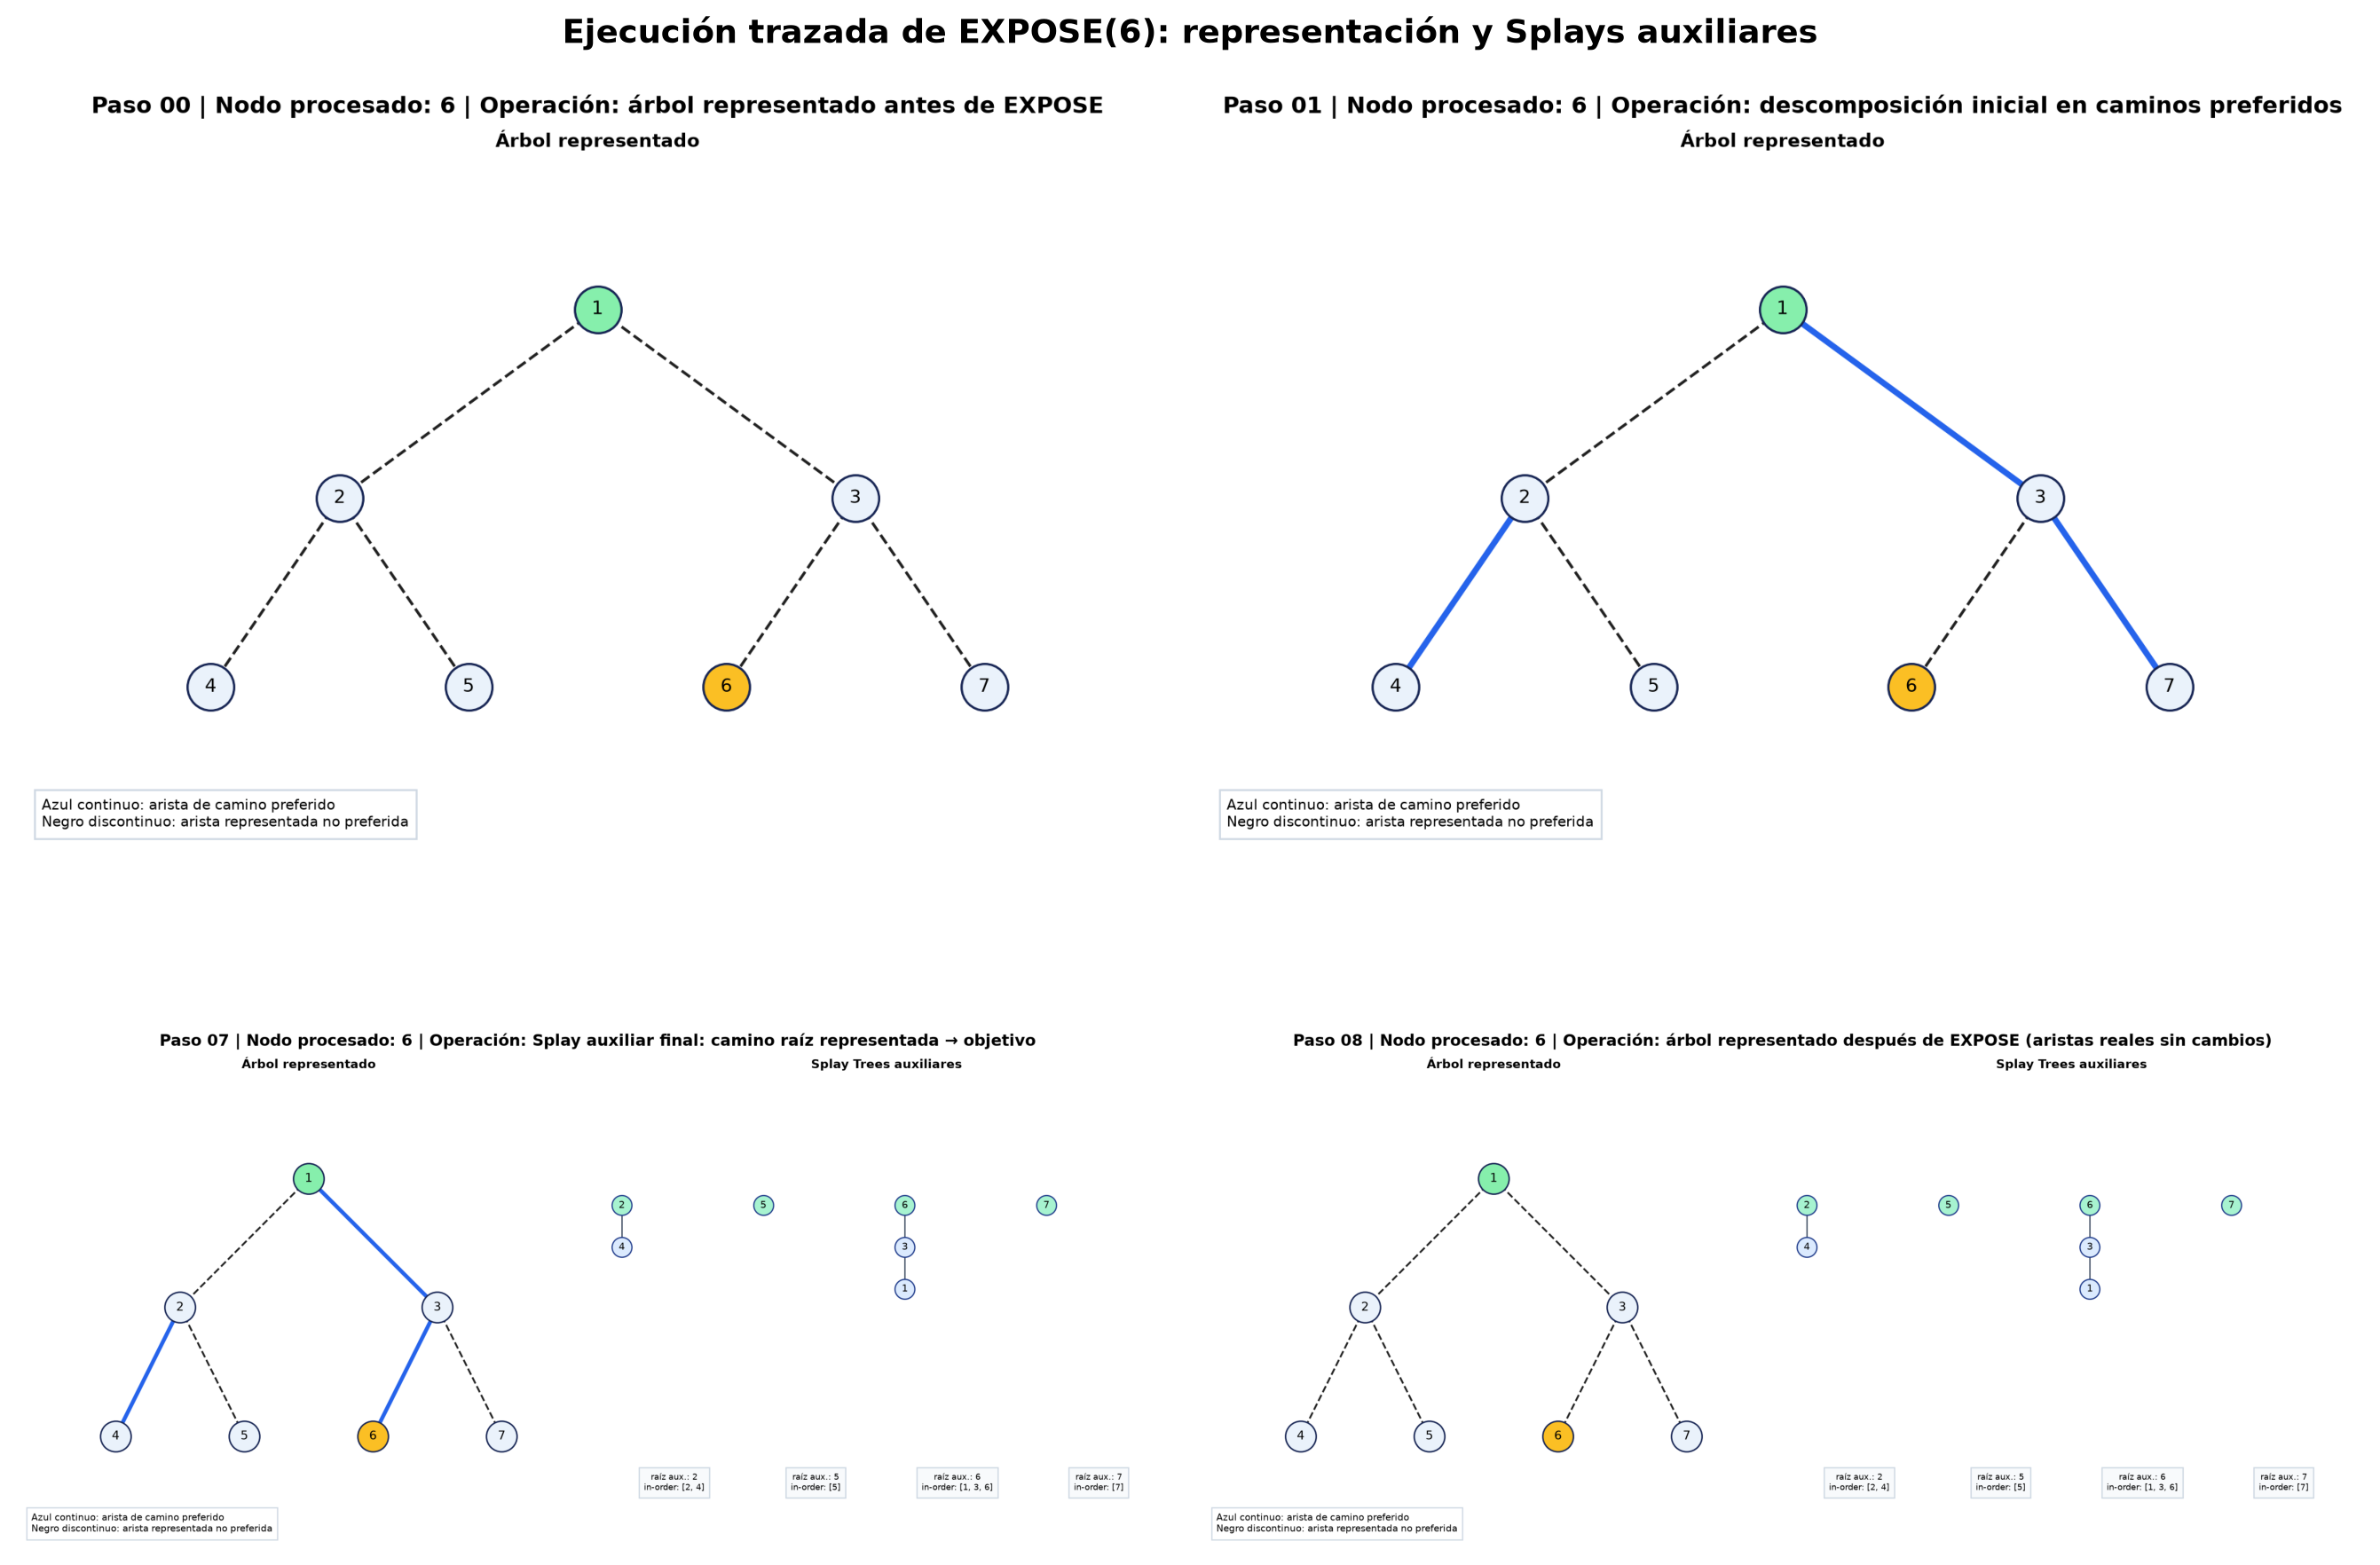
\includegraphics[width=\textwidth, keepaspectratio]{fig_expose_resumen.png}
    \caption{Visualización completa de las etapas de \texttt{EXPOSE(6)} según la guía}
    \label{fig:expose_resumen}
\end{figure}

\subsubsection*{Guion secuencial para la sustentación:}
\begin{enumerate}\setlength\itemsep{1pt}\setlength\parskip{0pt}
    \item \textbf{Paso 0 (Árbol representado antes):} Grafo lógico inicial con aristas directas $\{(1, 2), (1, 3), (2, 4), (2, 5), (3, 6), (3, 7)\}$.
    \item \textbf{Paso 1 (Descomposición en caminos preferidos):} Identifica las aristas sólidas activas antes de invocar expose.
    \item \textbf{Paso 2 (Árboles auxiliares antes):} Cada camino preferido reside en su propio Splay Tree con aristas discontinuas virtuales.
    \item \textbf{Pasos 3 al 6 (Splays y cambios de arista preferida):} Se aplica splay sobre $6$, se desconecta su hijo derecho hacia descendientes y se enlaza como hijo derecho el camino que desciende desde $3$ y $1$.
    \item \textbf{Paso 7 (Árbol auxiliar final):} El camino completo raíz $\to 6$ ($1 - 3 - 6$) queda en un único árbol Splay con $6$ en la raíz.
    \item \textbf{Paso 8 (Árbol representado después):} Confirma que las aristas del árbol lógico real \textbf{no cambiaron en absoluto}.
\end{enumerate}
